\subsection*{Problema 07}

\textbf{Enunciado:}
Calcular la integral indefinida:
\begin{align*}
I = \int \dfrac{\cos x \, dx}{5 + 4\cos x}
\end{align*}

\textbf{Solución:}
Siguiendo las indicaciones, reescribimos el numerador del integrando para descomponer la fracción original en dos partes más sencillas:
\begin{align*}
\cos x &= \dfrac{1}{4} \left( 5 + 4\cos x \right) - \dfrac{5}{4}
\end{align*}

Sustituyendo esta expresión en la integral:
\begin{align*}
I &= \int \dfrac{\frac{1}{4}(5 + 4\cos x) - \frac{5}{4}}{5 + 4\cos x} \, dx \\
I &= \dfrac{1}{4} \int dx - \dfrac{5}{4} \int \dfrac{dx}{5 + 4\cos x}
\end{align*}

La primera integral es inmediata:
\begin{align*}
I_1 &= \dfrac{1}{4} \int dx = \dfrac{x}{4}
\end{align*}

Para la segunda integral, denotada como $I_2$, aplicamos la sustitución de Weierstrass $z = \tan\left(\dfrac{x}{2}\right)$. Las identidades trigonométricas fundamentales son:
\begin{align*}
\cos x &= \dfrac{1 - z^2}{1 + z^2}, \quad dx = \dfrac{2 \, dz}{1 + z^2}
\end{align*}

Sustituyendo en $I_2$:
\begin{align*}
I_2 &= \dfrac{5}{4} \int \dfrac{\frac{2 \, dz}{1 + z^2}}{5 + 4\left(\dfrac{1 - z^2}{1 + z^2}\right)} \\
I_2 &= \dfrac{5}{2} \int \dfrac{dz}{5(1 + z^2) + 4(1 - z^2)} \\
I_2 &= \dfrac{5}{2} \int \dfrac{dz}{5 + 5z^2 + 4 - 4z^2} \\
I_2 &= \dfrac{5}{2} \int \dfrac{dz}{z^2 + 9}
\end{align*}

Esta última es una integral estándar del arco tangente:
\begin{align*}
I_2 &= \dfrac{5}{2} \left( \dfrac{1}{3} \arctan\left(\dfrac{z}{3}\right) \right) = \dfrac{5}{6} \arctan\left(\dfrac{z}{3}\right)
\end{align*}

Regresando a la variable original $x$:
\begin{align*}
I_2 &= \dfrac{5}{6} \arctan\left(\dfrac{\tan(x/2)}{3}\right)
\end{align*}

Combinando ambos resultados y añadiendo la constante de integración $C$:
\begin{align*}
I &= \dfrac{x}{4} - \dfrac{5}{6} \arctan\left(\dfrac{\tan(x/2)}{3}\right) + C
\end{align*}

\begin{figure}[H]
	\centering
	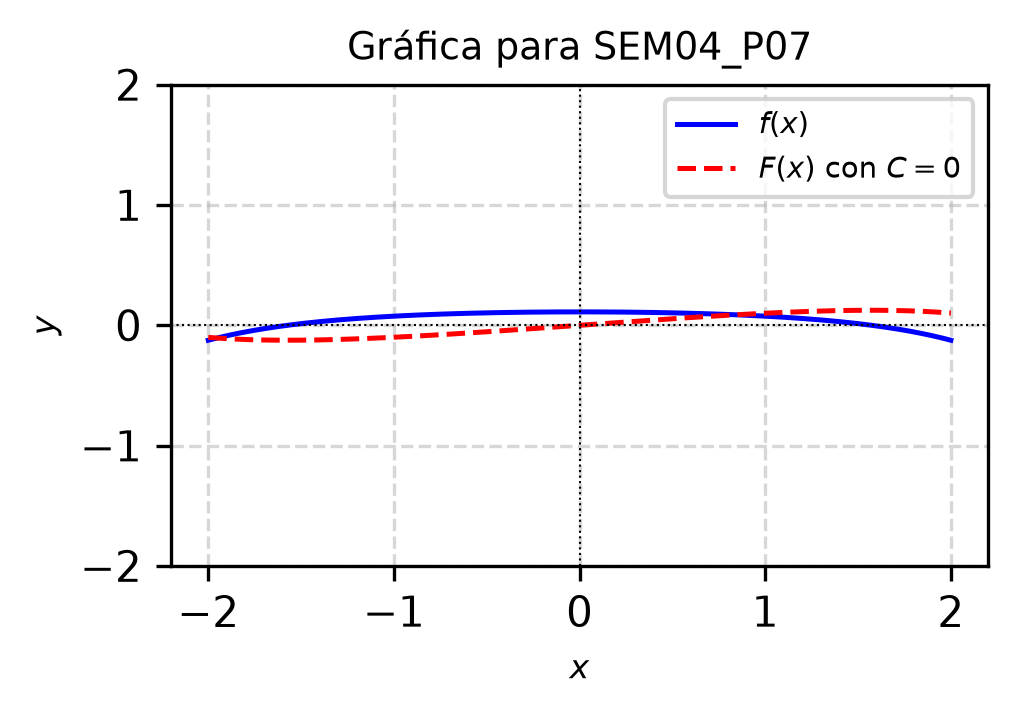
\includegraphics[width=\columnwidth]{semana_04/graficas/SEM04_P07_grafica.png}
	\caption{Representación gráfica de $f(x)$ y su antiderivada $F(x)$ evaluada para la constante de integración $C = 0$ (Problema 07).}
	\label{fig:problema07}
\end{figure}
